\documentclass[a4paper,14pt]{extarticle}

\usepackage[utf8x]{inputenc}
\usepackage[T1,T2A]{fontenc}
\usepackage[russian]{babel}
\usepackage{hyperref}
\usepackage{indentfirst}
\usepackage{here}
\usepackage{array}
\usepackage{graphicx}
\usepackage{caption}
\usepackage{subcaption}
\usepackage{chngcntr}
\usepackage{amsmath}
\usepackage{amssymb}
\usepackage{pgfplots}
\usepackage{pgfplotstable}
\usepackage[left=2cm,right=2cm,top=2cm,bottom=2cm,bindingoffset=0cm]{geometry}
\usepackage{multicol}
\usepackage{askmaps}
\usepackage{titlesec}
\usepackage{listings}
\usepackage{color}
\usepackage{courier}

\definecolor{green}{rgb}{0,0.6,0}
\definecolor{gray}{rgb}{0.5,0.5,0.5}
\definecolor{purple}{rgb}{0.58,0,0.82}

\lstset{
	language=Verilog,
	backgroundcolor=\color{white},   
	basicstyle=\small\ttfamily,
	commentstyle=\color{green},
	keywordstyle=\color{blue},	
	numberstyle=\tiny\color{gray},
	stringstyle=\color{purple},
	breakatwhitespace=false,
	breaklines=true,
	captionpos=b,
	keepspaces=true,
	numbers=left,
	numbersep=5pt,
	showspaces=false,
	showstringspaces=false,
	showtabs=false,
	tabsize=4,
	frame=single,
	inputpath={../quartus/},
	literate={~} {$\sim$}{1}
}

\renewcommand{\le}{\ensuremath{\leqslant}}
\renewcommand{\leq}{\ensuremath{\leqslant}}
\renewcommand{\ge}{\ensuremath{\geqslant}}
\renewcommand{\geq}{\ensuremath{\geqslant}}
\renewcommand{\epsilon}{\ensuremath{\varepsilon}}
\renewcommand{\phi}{\ensuremath{\varphi}}
\renewcommand{\thefigure}{\arabic{figure}} 	
\renewcommand*\not[1]{\overline{#1}}

\titleformat*{\section}{\large\bfseries} 
\titleformat*{\subsection}{\normalsize\bfseries} 
\titleformat*{\subsubsection}{\normalsize\bfseries} 
\titleformat*{\paragraph}{\normalsize\bfseries} 
\titleformat*{\subparagraph}{\normalsize\bfseries} 

\counterwithin{figure}{section}
\counterwithin{equation}{section}
\counterwithin{table}{section}
\newcommand{\sign}[1][5cm]{\makebox[#1]{\hrulefill}}
\graphicspath{{../pics/}}
\captionsetup{justification=centering,margin=1cm}
\def\arraystretch{1.3}
\setlength\parindent{5ex}
\titlelabel{\thetitle.\quad}

\begin{document}

\begin{titlepage}
\begin{center}
	Санкт-Петербургский Политехнический Университет Петра Великого\\[0.3cm]
	Институт компьютерных наук и технологий \\[0.3cm]
	Кафедра компьютерных систем и программных технологий\\[4cm]
	
	\textbf{ОТЧЕТ}\\ 
	\textbf{по лабораторной работе}\\[0.5cm]
	\textbf{SystemVerilog №4}\\[0.1cm]
	Автоматизация проектирования\\ дискретных устройств\\[4.0cm]
\end{center}

\begin{flushright}
	\begin{minipage}{0.45\textwidth}
		\textbf{Работу выполнил студент}\\[3mm]
		группа 33501/4 \hspace*{9mm} Дьячков В.В.\\[5mm]
		\textbf{Преподаватель}\\[5mm]
		\sign[1.5cm] \hspace*{1mm} к.т.н., доц. Филиппов А.С. \\[5mm]
	\end{minipage}
\end{flushright}

\vfill

\begin{center}
	Санкт-Петербург\\
	\the\year
\end{center}
\end{titlepage}

\addtocounter{page}{1}
\counterwithin{lstlisting}{section}

\tableofcontents
\listoffigures
\newpage

\section{Цель работы}

Познакомиться с базовыми возможностями встроенного логического анализатора SignalTapII пакета QuartusII. Научиться выполнять типовые действия для наблюдения и анализа сигналов в цифровых устройствах.

\section{Выполнение работы}

\subsection{Создание и ввод проекта}

На рис. \ref{fig:source} изображен исследуемый проект, обеспечивающий реализацию 27-разрядного счетчика, работающего на частоте 25 МГц, включение/выключение светодиодов \code{led[5..0]} старшими разрядами счетчика и соединение сигнала выхода переноса \code{cout} со светодиодом \code{led[6]}.

\begin{figure}[H]
	\begin{center}
		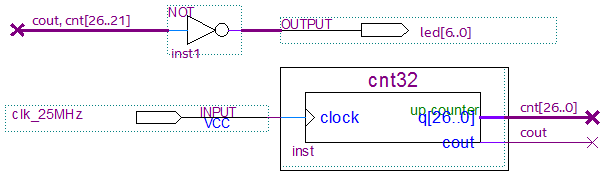
\includegraphics[width=0.7\textwidth]{source}
		\caption{Исследуемый проект}
		\label{fig:source}
	\end{center}
\end{figure}
\vspace{-1cm}

\subsection{Создание экземпляра логического анализатора ELA1}

На рис. \ref{fig:stp_1} изображено окно SignalTapII Logic Analyzer со списком целей в созданном \code{stp}-файле.
\vspace{-0.5cm}
\begin{figure}[H]
	\begin{center}
		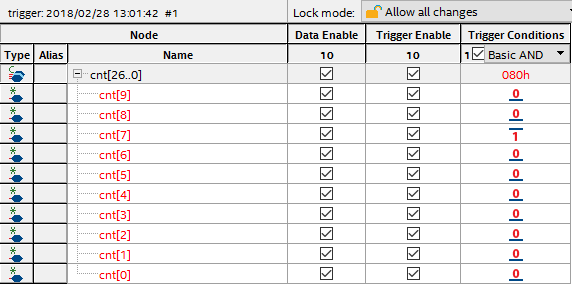
\includegraphics[width=0.8\textwidth]{stp_1}
		\caption{Список целей в SignalTapII Logic Analyzer}
		\label{fig:stp_1}
	\end{center}
\end{figure}

\subsection{Конфигурирование СБИС}

На рис. \ref{fig:stp_2} изображено окно SignalTapII Logic Analyzer после конфигурации и программирования СБИС.

\begin{figure}[H]
	\begin{center}
		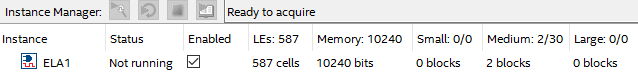
\includegraphics[width=0.95\textwidth]{stp_2}
		\caption{Список целей в SignalTapII Logic Analyzer}
		\label{fig:stp_2}
	\end{center}
\end{figure}

\subsection{Захват и анализ данных}

На рис. \ref{fig:data_1} изображены захваченные данные в SignalTapII Logic Analyzer, записанные когда значение разрядов счетчика \code{cnt[9..0]} станет равным \code{128}.

\begin{figure}[H]
	\begin{center}
		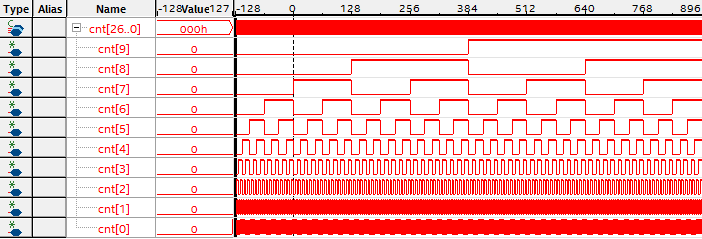
\includegraphics[width=0.95\textwidth]{data_1}
		\caption{Захваченные данные r}
		\label{fig:data_1}
	\end{center}
\end{figure}

На рис. \ref{fig:data_2} захваченные данные изображены в формате \code{Unsigned Bar Chart}.

\begin{figure}[H]
	\begin{center}
		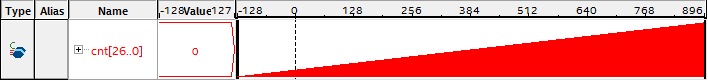
\includegraphics[width=0.95\textwidth]{data_2}
		\caption{Захваченные данные в формате Unsigned Bar Chart}
		\label{fig:data_2}
	\end{center}
\end{figure}

\subsection{Управление режимами захвата данных}

На рис. \ref{fig:data_3} захваченные данные изображены с \code{Trigger position = Center trigger position} и значением условия захвата данных равным \code{128}.

\vspace{-0.5cm}
\begin{figure}[H]
	\begin{center}
		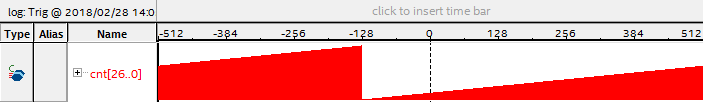
\includegraphics[width=0.95\textwidth]{data_3}
		\caption{Захваченные данные с Center trigger position (\code{128})}
		\label{fig:data_3}
	\end{center}
\end{figure}

На рис. \ref{fig:data_4} захваченные данные изображены с \code{Trigger position = Center trigger position} и значением условия захвата данных равным \code{512}.

\vspace{-0.5cm}
\begin{figure}[H]
	\begin{center}
		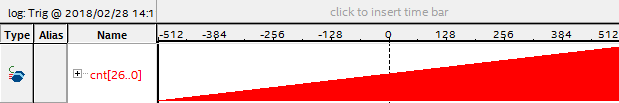
\includegraphics[width=0.95\textwidth]{data_4}
		\caption{Захваченные данные с Center trigger position (\code{512})}
		\label{fig:data_4}
	\end{center}
\end{figure}

На рис. \ref{fig:data_5} захваченные данные изображены с \code{Trigger position = Post trigger position} и значением условия захвата данных равным \code{128}.

\vspace{-0.5cm}
\begin{figure}[H]
	\begin{center}
		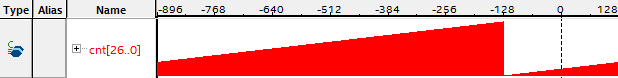
\includegraphics[width=0.95\textwidth]{data_5}
		\caption{Захваченные данные с Post trigger position (\code{128})}
		\label{fig:data_5}
	\end{center}
\end{figure}

На рис. \ref{fig:data_6} захваченные данные изображены с \code{Trigger position = Post trigger position} и значением условия захвата данных равным \code{896}.

\vspace{-0.5cm}
\begin{figure}[H]
	\begin{center}
		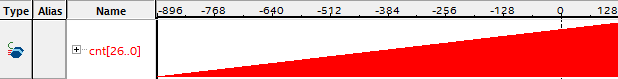
\includegraphics[width=0.95\textwidth]{data_6}
		\caption{Захваченные данные с Post trigger position (\code{896})}
		\label{fig:data_6}
	\end{center}
\end{figure}

На рис. \ref{fig:data_7} захваченные данные изображены с сегментированным типом буфера (4 сегмента по 256 отсчетов) и \code{Trigger position = Center trigger position}.

\vspace{-0.5cm}
\begin{figure}[H]
	\begin{center}
		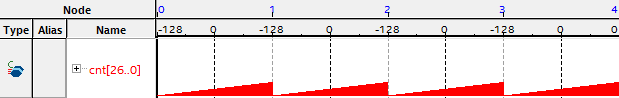
\includegraphics[width=0.95\textwidth]{data_7}
		\caption{Захваченные данные с Post trigger position (\code{896})}
		\label{fig:data_7}
	\end{center}
\end{figure}

\section{Дополнительное задание}

Сигнал переноса \code{cout} выведен на светодиод \code{led[6]}, однако он не загорается. Это можно объяснить тем, что сигнал переноса появляется только на один такт и кажется, что светодиод не загорается.

На рис. \ref{fig:data_8} изображены снятые данные для сигналов \code{cnt[26..21]} и сигнала переноса \code{cout} в новом экземпляре логического анализатора \code{ELA2}. Из временной диаграммы видно, что на один такт \code{led[6] = 0}, что соответствует значению \code{cout = 1}.

\vspace{-0.5cm}
\begin{figure}[H]
	\begin{center}
		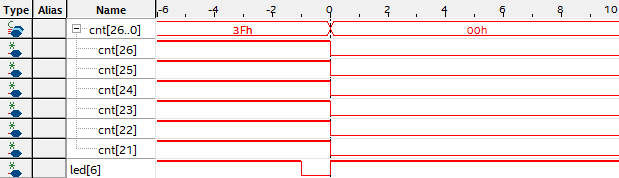
\includegraphics[width=0.95\textwidth]{data_8}
		\caption{Захваченные данные с Post trigger position (\code{896})}
		\label{fig:data_8}
	\end{center}
\end{figure}

\section{Выводы}

В ходе работы изучены основы работы с встроенным логическим анализатором \code{SignalTapII} пакета \code{QuartusII}. Были созданы два экземпляра анализатора для получения временных диаграмм для сигналов старших и младших разрядов. Рассмотрены различные режимы захвата данных с различными значениями \code{Triger position} и типа буфера. Временные диаграммы, построенные по захваченным данным, позволили проанализировать сигналы в цифровых устройствах.

\end{document}